\section{Introduction}

\subsection{Motivation}
\begin{frame}[label=Motivation]
\frametitle{Motivation}
\begin{enumerate}
  \item<1> Interest in using MHD models for operational forecasting;
  very little validation is done.
  \begin{itemize}
    \item Most common: in-situ data analysis.
    \item Comprehensive inter-model comparison is not done.
  \end{itemize}
  \item<2> Want understanding of MHD magnetosphere sensitivity to
  initial solar wind conditions.
  \begin{itemize}
    \item Sensitivities not looked into yet.
  \end{itemize}
  \item<3> Want a better understanding of MHD model differences.
  \begin{itemize}
	\item New tool in analyzing two model outputs: Differences.
  \end{itemize}
\end{enumerate}
\end{frame}

% Difficult to model the magnetosphere over an 11 year cycle today, GEM
% challenge is only 6-8 events, each event is unique, documenting the tendencies
% of models gives a reference to model developers as to why a model does poorly
\begin{frame}[label=Summary]
\frametitle{Summary}
\begin{enumerate}
  \item This new inter-model difference comparison, with future work will offer
  a new perspective to model developers in understanding reasoning behind
  results from in-situ data analysis.
  \item MHD models are very sensitive in response to initial conditions. Found
  regions of inconsistencies in these numerical models. For example high
  compression gave three very different results.
  \item Differences between models are large. The ring current has an effect on
  the BATS-R-US output and more validation is still needed to determine the causes
  of these differences. For example, changes in preconditioning times.
\end{enumerate}

\end{frame}


\subsection{Experiments}
\begin{frame}[label=Experiments]
\frametitle{Experiments}
\begin{enumerate}
  \item Response to a change in solar wind $B_z$ from positive to negative.
  (Addresses all motivations)
  \item The influence of preconditioning on MHD magnetospheric models.
  (Addresses motivations 1 and 3)
  \item How magnetospheric MHD models differ in their response to
  extreme solar wind conditions. (Addresses all motivations)
\end{enumerate}
\end{frame}


\subsection{Space Weather}
\begin{frame}
\frametitle{Space Weather}
\centering 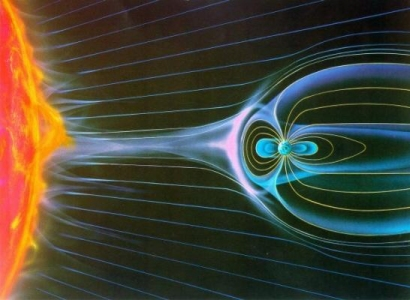
\includegraphics[scale=0.3]{images/NASA_BigPicture.jpg}

\textbf{Space weather:} The term used to describe the current state of the
space environment involving the influence of particles traveling outward from the Sun
on objects in the heliosphere, magnetosphere, ionosphere and thermosphere
(Thompson, 2000)

\end{frame}